% Group report: Network Security project on a private Tor network.
% Structure from the professor's template (main (1).pdf, section 4): title page,
% group and activity description, introduction, the group work, conclusions,
% bibliography, appendices with "who did what".
% Compile with:  latexmk -pdf main.tex

\documentclass[10pt,a4paper]{article}

\usepackage[T1]{fontenc}
\usepackage[margin=0.75in]{geometry}
\usepackage{amsmath}
\usepackage{amssymb}
\usepackage{graphicx}
\usepackage{booktabs}
\usepackage{listings}
\usepackage{titlesec}
\usepackage{float}
\usepackage{hyperref}

\titleformat{\section}{\large\bfseries}{\thesection.}{0.5em}{}
\titlespacing*{\section}{0pt}{1.0ex}{0.3ex}

\setlength{\parindent}{0pt}
\setlength{\parskip}{0.4em}
\linespread{1.03}

% Figures and tables numbered by section ("Fig. 3.1"), as in the style notes.
\numberwithin{figure}{section}
\numberwithin{table}{section}
\graphicspath{{figures/}}

\lstset{basicstyle=\ttfamily\small, breaklines=true, columns=fullflexible}

\hypersetup{
    colorlinks=true,
    linkcolor=black,
    citecolor=black,
    urlcolor=blue
}

% TODO (group): final title and group name.
\title{\textbf{Traffic Correlation on a Private Tor Network}}
\author{Daniel Carpitella, Elena Pozzebon, Sebastiano Boato\\
Group: TODO\\
Network Security -- Ca' Foscari University of Venice, A.Y.\ 2025/2026}
\date{}

\begin{document}

\maketitle

\begin{abstract}
\normalsize
% TODO (group): abstract, to be written at the end.
\end{abstract}
\newpage

\section{Group and Activity Description}
\label{sec:group}
% TODO (group): the members of the group and how the work was split
% (professor's template, section 4.2). Details in Appendix~\ref{app:who-did-what}.
\section{Introduction}
\label{sec:introduction}
% TODO (group), from the professor's template (section 4.2.1):
% - goals of the project;
% - why it is important;
% - what we did in a nutshell.
\section{Background}
\label{sec:background}
% TODO (group): Tor circuits (guard, middle, exit), onion services, traffic
% correlation attacks, conflux. Every statement needs a reference (style notes).
\section{Private Tor Network}
\label{sec:lab}
% TODO (group): the lab shared by all experiments (docker/, cli/, shared-base/):
% directory authorities, relays, exits, client, targets, Tor version.
\section{(DRAFT TEMPORANEO, tutto da rivedre)Clearnet Correlation: Client Guard and Exit Relay}
\label{sec:clearnet}
% Author: Daniel Carpitella. Sources in experiments/clearnet-correlation/:
% README.md for the design choices, clearnet_analysis.ipynb for the results.
% Status: draft, to be reviewed.

\subsection{Goal and Threat Model}
\label{sec:clearnet-goal}

When a Tor client contacts a server outside the Tor network, its traffic leaves
the network at an exit relay. The Guard knows the address of the client but not
the destination, while the Exit knows the destination but not the client. An
observer that sees both sides can still try to link them by comparing the timing
of the traffic. This end-to-end correlation is outside what Tor claims to
prevent~\cite{dingledine2004tor}.

This experiment measures how well such an observer performs in our private
network. The observer sees two links:
\begin{itemize}
    \item \textbf{Guard side:} the packets between the client and its Guard, on
    the relay port 9001, encrypted with TLS;
    \item \textbf{Exit side:} the packets between the Exit and the web server, in
    plain HTTP on port 80.
\end{itemize}
The observer uses only the timestamp, the size and the direction of each packet.
It decrypts nothing and has no access to the logs of the client or of the
server: these logs are used only afterwards, to check which requests the
observer has recognised. The experiment complements the onion one
(Section~\ref{sec:onion}), where the observer watches the Guards of the client
and of the onion service.

\subsection{Experimental Setup}
\label{sec:clearnet-setup}

\textbf{Target.} The lab of Section~\ref{sec:lab} is extended with a web server
(Python \texttt{http.server}) on a separate Docker network. The Exits are the only
relays attached to that network, so the client can reach the server only through
Tor, and the server sees as TCP peer the address of the Exit that forwarded the
request.

\textbf{Workload.} We ran 5 runs of 100 sequential requests each. The client
fetches the same page, a file of 10\,000 random bytes, with \texttt{curl} through
the SOCKS5 port of the Tor client. Between two requests it waits a random pause,
uniform between 2 and 5\,s, as in the onion experiment; each run lasts about
6 minutes. Each URL carries a unique request ID. The client records the start, the
end and the outcome of each request, and the server log records the ID together
with the address of the Exit. The page size follows from the burst threshold of
the method (1000 bytes, Section~\ref{sec:clearnet-method}): the default test page
of the lab, about 30 bytes, would produce no burst at all on the Exit side.

\textbf{Client configuration.} The client keeps the default Tor configuration:
Guards and Exits are not pinned and conflux is active. With conflux the client
builds two circuits, called legs, that start from different Guards and end at the
same Exit, and it can send traffic on either of them~\cite{alsabah2013path}. The
recorded circuit events show linked conflux circuits in every run. Pinning the
nodes would require a modified client (fixed entry and exit nodes, conflux
disabled), which no longer behaves like a normal one. It is also not needed to
measure the correlation: the actual-path analysis of
Section~\ref{sec:clearnet-method} evaluates each request with the nodes it really
used.

\textbf{Capture.} During each run \texttt{tcpdump} captures the traffic of all the
11 relays: on port 9001, and on the Exits also the traffic with the server. Each
capture is exported with \texttt{tshark} to a table with timestamp, frame size,
addresses and ports, and is cut to the interval from 5\,s before the first
request to 5\,s after the last one. In parallel, the circuit and stream events of
the client are recorded through its control port, as a cross-check of the paths.

\textbf{Data check.} All 500 requests returned HTTP 200 to the client, and each
request ID appears exactly once in the server log. \texttt{tcpdump} reported no
dropped packet. All the analyses use the 500 requests confirmed by the server.

\subsection{Correlation Method}
\label{sec:clearnet-method}

The method and its parameters are the same as in the onion experiment
(Section~\ref{sec:onion}), so that the two sets of numbers can be compared.

\begin{itemize}
    \item \textbf{Bursts.} On each link, consecutive packets in the same direction
    with gaps of at most 100\,ms form a burst. A packet in the opposite
    direction closes the burst, pure TCP acknowledgements included. Bursts below
    1000 bytes are discarded, and only the start time of a burst is used.
    \item \textbf{Pairs.} Each Guard burst, in time order, is paired with the
    closest unused Exit burst that starts within $\pm 50$\,ms. Each burst belongs
    to at most one pair.
    \item \textbf{Covered request.} A request is covered if the Guard burst of at
    least one pair starts in $[t_s - 50\,\text{ms},\ t_e + 50\,\text{ms}]$, where
    $t_s$ and $t_e$ are the start and the end of the request recorded by the
    client. Seen from the client, a request lasts 25\,ms (median; 16--38\,ms
    between the 5th and the 95th percentile).
    \item \textbf{Control.} The Guard bursts of run $i$ are paired with the Exit
    bursts of another run $j$, shifted so that the first requests of the two runs
    coincide. No real pair can exist between different runs, so the result
    measures the pairs that appear by chance. The control value of a run is the
    mean over the other four runs.
\end{itemize}

\textbf{Links.} On the Guard side we keep only the packets exchanged between the
Guard and the client, and on the Exit side only those exchanged between the Exit
and the server. The rest of the Guard traffic does not add information about the
client. The Guard--middle link carries the same cells a few milliseconds apart,
and the traffic of other circuits and of the directory forms bursts that cannot
match the requests. The filter is within reach of a real observer, because the
link of the client is the one that carries its address. It also removes the
copies of packets of other hosts that the Docker bridge sometimes delivers to a
capture. The onion analysis used all the traffic on port 9001 of the two Guards
instead. Section~\ref{sec:clearnet-results} reports both variants.

\textbf{Actual path.} Each request is evaluated with the Guard and the Exit it
really used. The Exit is the one whose address the server logged for the
request. The Guard is the relay that exchanged the most bytes with the client
during the request. The Guard is taken from the captures rather than from the
client log, because with conflux the client log names only one of the two legs.
For every Guard--Exit combination used in a run the two traces are paired, and a
request counts as covered only by pairs of its own combination. This is the
measure that an experiment with pinned nodes would give. It describes an observer
that controls the Guard and the Exit of every request. An observer that controls
a single Guard and a single Exit is discussed in
Section~\ref{sec:clearnet-visibility}.

\subsection{Results Comparable with the Onion Experiment}
\label{sec:clearnet-results}

\textbf{Paths.} All 500 requests left the network through the same Exit. The
response of each request crossed one of two Guards, the two legs of conflux, and
the split changes from run to run (Table~\ref{tab:clearnet-guards}). In the lab
both Guards are directory authorities, which also act as relays.

\begin{table}[htb]
\centering
\caption{Requests per Guard in the actual-path analysis. All requests used the same Exit.}
\label{tab:clearnet-guards}
\begin{tabular}{lrrrrr}
\toprule
Guard & Run 1 & Run 2 & Run 3 & Run 4 & Run 5 \\
\midrule
\texttt{dasikrbniw} & 94 & 49 & 0 & 58 & 75 \\
\texttt{daythqtcja} & 6 & 51 & 100 & 42 & 25 \\
\bottomrule
\end{tabular}
\end{table}

\textbf{Correlation.} Figure~\ref{fig:clearnet-actual} shows the result per run,
and Table~\ref{tab:clearnet-comparison} the totals. Every request is covered:
500 out of 500, against 4.1\% in the control. When the observer watches the
Guard and the Exit that a request really used, timing alone links the two sides
of every request.

On the bursts, 81.8\% of the 986 Guard bursts find a partner, against 3.5\% by
chance; on the Exit side 80.9\% of 998 bursts, against 3.4\%. All the Guard
bursts left without a partner fall inside a request and go from the Guard to the
client, so they are pieces of a response. The same response splits into more
bursts on the Guard side than on the Exit side: in run 1, the 94 responses that
crossed \texttt{dasikrbniw} form 249 bursts on its link with the client, while
each response forms 2 bursts on the Exit link. Since the pairing is one-to-one,
the extra pieces remain without a partner.

\begin{figure}[htb]
\centering
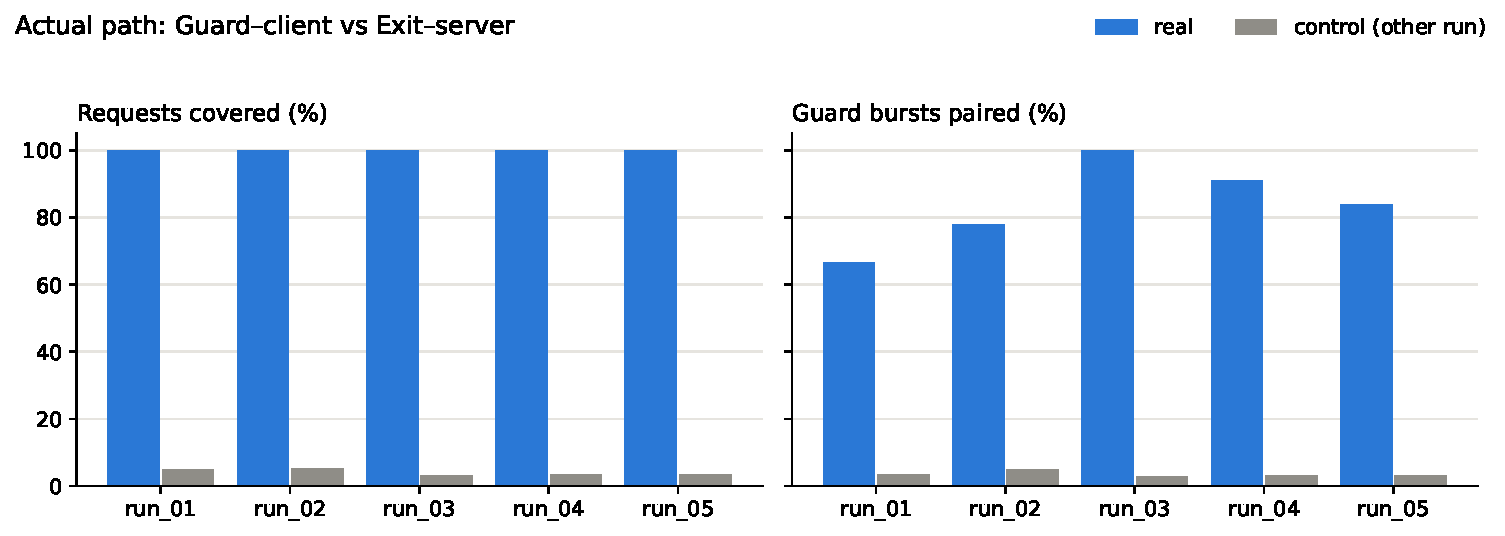
\includegraphics[width=\linewidth]{../experiments/clearnet-correlation/figures/a1_actual_path.pdf}
\caption{Actual-path analysis, per run: requests covered and Guard bursts with a
partner, for the real data and for the cross-run control.}
\label{fig:clearnet-actual}
\end{figure}

\begin{table}[htb]
\centering
\caption{Totals over the 5 runs. Control values in parentheses. Onion values from
Section~\ref{sec:onion}.}
\label{tab:clearnet-comparison}
\begin{tabular}{lrrr}
\toprule
 & Clearnet & Clearnet & Onion \\
 & Guard--client link & all Guard traffic & two Guards \\
\midrule
Guard bursts with a partner & 81.8\% of 986 (3.5\%) & 48.8\% of 2756 (2.0\%) & 54.8\% of 1405 (2.4\%) \\
Requests covered & 500/500 (4.1\%) & 500/500 (4.1\%) & 429/500 (3.1\%) \\
\bottomrule
\end{tabular}
\end{table}

\textbf{Comparison with the onion experiment.} With all the Guard traffic, as in
the onion analysis, the Guard capture holds 2.8 times as many bursts and the
share of paired Guard bursts drops from 81.8\% to 48.8\%. Request coverage does
not change. Computed in the same way, the share of paired bursts is close to the
onion one (48.8\% against 54.8\%), with a similar control. Request coverage is
higher than in the onion experiment, 100\% against 85.8\%. In the onion
experiment the uncovered requests are explained by the 1000-byte threshold
applied to a page of a few bytes, while here the page is 10\,KB. The difference
therefore reflects the page more than the scenario.

The two experiments also differ in the observed links (Guard--client and
Exit--server here, two Guards in the onion case). They differ in the nodes as
well: here each request is evaluated with the nodes it actually used, while the
onion analysis watched two fixed Guards. As in the onion experiment, there is
only one client and one server. The figures show that the two sides are linked in
time, not that the observer could pick the right pair among many concurrent
flows.

\subsection{Observed Nodes and Visibility}
\label{sec:clearnet-visibility}
% TODO: notebook, part B (attacker that controls one Guard and one Exit).

\subsection{Effect of Conflux}
\label{sec:clearnet-conflux}
% TODO: notebook, part B.

\subsection{Sensitivity to TCP Acknowledgements}
\label{sec:clearnet-acks}
% TODO: notebook, part B.

\subsection{Limitations}
\label{sec:clearnet-limits}
% TODO: 3 exits only; latency of a few milliseconds; packets not segmented between
% containers (offloading). See the README, "Dopo i run".
\section{Onion Service Correlation}
\label{sec:onion}
% TODO (Elena Pozzebon): experiments/onion-correlation/.
\section{Topology Comparison}
\label{sec:topology}
% TODO (Sebastiano Boato): experiments/topology-comparison/.
\section{Conclusions}
\label{sec:conclusions}
% TODO (group): what we have learned (professor's template, section 4.4).

% TODO (group): the professor's how-to has an "Evaluation Page" to leave as it is.
% Check the template source on Moodle and add it here if it belongs to the report.

% Bibliography. The style notes require every entry to be cited in the text.
\bibliographystyle{IEEEtran}
\bibliography{references}

\appendix
\section{Who Did What}
\label{app:who-did-what}
% TODO (group): required by the professor's checklist.
\section{Reproducing the Experiments}
\label{app:reproducibility}
% TODO (group): code fragments, configuration files and commands needed to reproduce
% the experiments (professor's template). Code as real listings, not screenshots.

\end{document}
